\documentclass{standalone}
\usepackage{tikz}
\usetikzlibrary{patterns, positioning}
\usepackage[sfdefault]{ClearSans} %% option 'sfdefault' activates Clear Sans as the default text font
\usepackage[T1]{fontenc}

\begin{document}
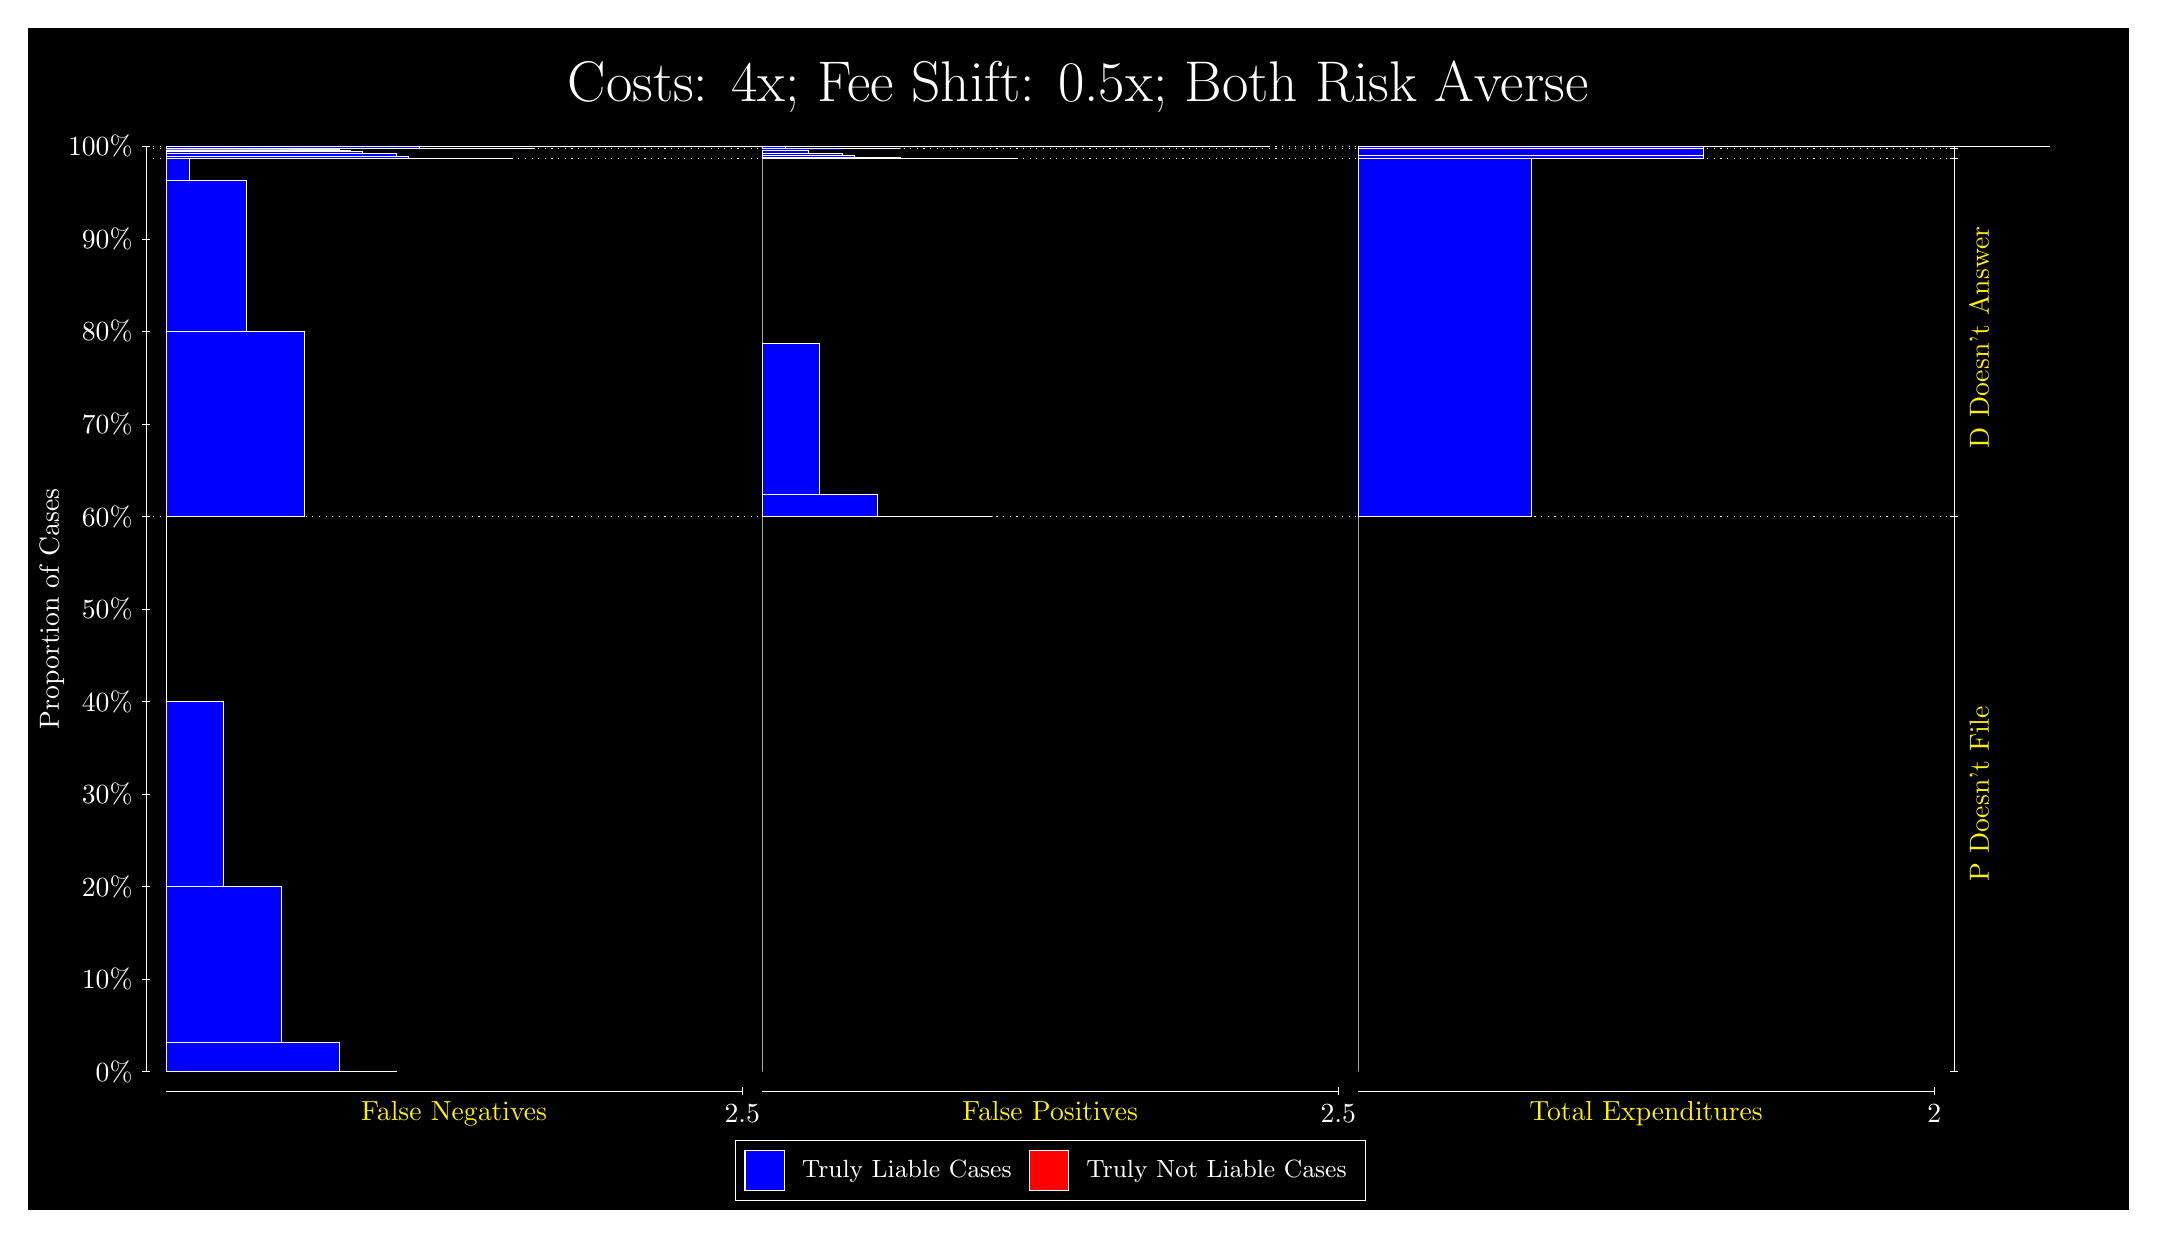
\begin{tikzpicture}
\draw[fill=black] (0,0) rectangle (26.667,15);
\draw[text=white] (0,13.5) rectangle (26.667,15) node[midway] {\huge Costs: 4x; Fee Shift: 0.5x; Both Risk Averse};
\draw[white, very thin] (1.5,1.75) -- (1.5,13.5);
\node[rotate=90, text=white, anchor=center] at (0.3, 7.625) {Proportion of Cases};
\draw[white, very thin] (1.45,1.75) -- (1.55,1.75);
\node[text=white, anchor=east] at (1.45, 1.75) {0\%};
\draw[white, very thin] (1.45,2.925) -- (1.55,2.925);
\node[text=white, anchor=east] at (1.45, 2.925) {10\%};
\draw[white, very thin] (1.45,4.1) -- (1.55,4.1);
\node[text=white, anchor=east] at (1.45, 4.1) {20\%};
\draw[white, very thin] (1.45,5.275) -- (1.55,5.275);
\node[text=white, anchor=east] at (1.45, 5.275) {30\%};
\draw[white, very thin] (1.45,6.45) -- (1.55,6.45);
\node[text=white, anchor=east] at (1.45, 6.45) {40\%};
\draw[white, very thin] (1.45,7.625) -- (1.55,7.625);
\node[text=white, anchor=east] at (1.45, 7.625) {50\%};
\draw[white, very thin] (1.45,8.8) -- (1.55,8.8);
\node[text=white, anchor=east] at (1.45, 8.8) {60\%};
\draw[white, very thin] (1.45,9.975) -- (1.55,9.975);
\node[text=white, anchor=east] at (1.45, 9.975) {70\%};
\draw[white, very thin] (1.45,11.15) -- (1.55,11.15);
\node[text=white, anchor=east] at (1.45, 11.15) {80\%};
\draw[white, very thin] (1.45,12.325) -- (1.55,12.325);
\node[text=white, anchor=east] at (1.45, 12.325) {90\%};
\draw[white, very thin] (1.45,13.5) -- (1.55,13.5);
\node[text=white, anchor=east] at (1.45, 13.5) {100\%};

\draw[white, very thin] (24.457,1.75) -- (24.457,13.5);
\draw[white, very thin] (24.407,1.75) -- (24.507,1.75);
\node[anchor=west] at (24.407, 1.75) {};
\draw[white, very thin] (24.407,8.8012) -- (24.507,8.8012);
\node[anchor=west] at (24.407, 8.8012) {};
\draw[white, very thin] (24.407,13.347) -- (24.507,13.347);
\node[anchor=west] at (24.407, 13.347) {};
\draw[white, very thin] (24.407,13.471) -- (24.507,13.471);
\node[anchor=west] at (24.407, 13.471) {};
\draw[white, very thin] (24.407,13.499) -- (24.507,13.499);
\node[anchor=west] at (24.407, 13.499) {};
\draw[white, very thin] (24.407,13.5) -- (24.507,13.5);
\node[anchor=west] at (24.407, 13.5) {};

\draw[white, very thin, fill=blue] (1.75,1.75) rectangle (4.6775,1.7538);
\draw[white, very thin, fill=blue] (1.75,1.7538) rectangle (3.9457,2.1271);
\draw[white, very thin, fill=blue] (1.75,2.1271) rectangle (3.2138,4.1043);
\draw[white, very thin, fill=blue] (1.75,4.1043) rectangle (2.4819,6.4512);
\draw[white, very thin, fill=red] (1.75,6.4512) rectangle (1.75,6.4512);
\draw[white, very thin, fill=blue] (1.75,6.4512) rectangle (1.75,8.8012);
\draw[white, very thin, fill=blue] (1.75,8.8012) rectangle (3.5065,11.147);
\draw[white, very thin, fill=blue] (1.75,11.147) rectangle (2.7746,13.073);
\draw[white, very thin, fill=blue] (1.75,13.073) rectangle (2.0428,13.347);
\draw[white, very thin, fill=red] (1.75,13.347) rectangle (1.75,13.347);
\draw[white, very thin, fill=blue] (1.75,13.347) rectangle (1.75,13.347);
\draw[white, very thin, fill=blue] (1.75,13.347) rectangle (6.1413,13.347);
\draw[white, very thin, fill=blue] (1.75,13.347) rectangle (5.5558,13.347);
\draw[white, very thin, fill=blue] (1.75,13.347) rectangle (5.4094,13.351);
\draw[white, very thin, fill=blue] (1.75,13.351) rectangle (4.9703,13.351);
\draw[white, very thin, fill=blue] (1.75,13.351) rectangle (4.8239,13.373);
\draw[white, very thin, fill=blue] (1.75,13.373) rectangle (4.6775,13.412);
\draw[white, very thin, fill=blue] (1.75,13.412) rectangle (4.2384,13.434);
\draw[white, very thin, fill=blue] (1.75,13.434) rectangle (4.092,13.456);
\draw[white, very thin, fill=blue] (1.75,13.456) rectangle (3.9457,13.457);
\draw[white, very thin, fill=blue] (1.75,13.457) rectangle (3.5065,13.471);
\draw[white, very thin, fill=blue] (1.75,13.471) rectangle (3.3602,13.471);
\draw[white, very thin, fill=blue] (1.75,13.471) rectangle (3.2138,13.471);
\draw[white, very thin, fill=blue] (1.75,13.471) rectangle (2.7746,13.471);
\draw[white, very thin, fill=blue] (1.75,13.471) rectangle (2.6283,13.471);
\draw[white, very thin, fill=blue] (1.75,13.471) rectangle (2.0428,13.471);
\draw[white, very thin, fill=red] (1.75,13.471) rectangle (1.75,13.471);
\draw[white, very thin, fill=blue] (1.75,13.471) rectangle (6.4341,13.471);
\draw[white, very thin, fill=blue] (1.75,13.471) rectangle (5.7022,13.474);
\draw[white, very thin, fill=blue] (1.75,13.474) rectangle (4.9703,13.498);
\draw[white, very thin, fill=blue] (1.75,13.498) rectangle (4.2384,13.499);
\draw[white, very thin, fill=blue] (1.75,13.499) rectangle (3.5065,13.499);
\draw[white, very thin, fill=red] (1.75,13.499) rectangle (1.75,13.499);
\draw[white, very thin, fill=blue] (1.75,13.499) rectangle (9.9471,13.499);
\draw[white, very thin, fill=blue] (1.75,13.499) rectangle (9.2152,13.499);
\draw[white, very thin, fill=blue] (1.75,13.499) rectangle (8.4834,13.499);
\draw[white, very thin, fill=blue] (1.75,13.499) rectangle (7.7515,13.499);
\draw[white, very thin, fill=blue] (1.75,13.499) rectangle (7.4587,13.499);
\draw[white, very thin, fill=blue] (1.75,13.499) rectangle (7.0196,13.499);
\draw[white, very thin, fill=blue] (1.75,13.499) rectangle (6.7268,13.499);
\draw[white, very thin, fill=blue] (1.75,13.499) rectangle (5.9949,13.499);
\draw[white, very thin, fill=blue] (1.75,13.499) rectangle (5.2631,13.5);
\draw[white, very thin, fill=blue] (1.75,13.5) rectangle (4.5312,13.5);
\draw[white, very thin, fill=blue] (1.75,13.5) rectangle (3.7993,13.5);
\draw[white, very thin, fill=blue] (1.75,13.5) rectangle (3.0674,13.5);
\draw[white, very thin, fill=blue] (1.75,13.5) rectangle (2.3355,13.5);
\draw[white, very thin, fill=red] (1.75,13.5) rectangle (1.75,13.5);
\draw[white, very thin, fill=red] (9.3189,1.75) rectangle (9.3189,1.75);
\draw[white, very thin, fill=blue] (9.3189,1.75) rectangle (9.3189,8.8012);
\draw[white, very thin, fill=red] (9.3189,8.8012) rectangle (12.246,8.8012);
\draw[white, very thin, fill=blue] (9.3189,8.8012) rectangle (12.246,8.8012);
\draw[white, very thin, fill=blue] (9.3189,8.8012) rectangle (11.515,8.8016);
\draw[white, very thin, fill=blue] (9.3189,8.8016) rectangle (10.783,9.0759);
\draw[white, very thin, fill=blue] (9.3189,9.0759) rectangle (10.051,11.002);
\draw[white, very thin, fill=blue] (9.3189,11.002) rectangle (9.3189,13.347);
\draw[white, very thin, fill=red] (9.3189,13.347) rectangle (12.539,13.347);
\draw[white, very thin, fill=blue] (9.3189,13.347) rectangle (12.539,13.347);
\draw[white, very thin, fill=red] (9.3189,13.347) rectangle (11.954,13.347);
\draw[white, very thin, fill=blue] (9.3189,13.347) rectangle (11.954,13.347);
\draw[white, very thin, fill=blue] (9.3189,13.347) rectangle (11.807,13.347);
\draw[white, very thin, fill=red] (9.3189,13.347) rectangle (11.368,13.347);
\draw[white, very thin, fill=blue] (9.3189,13.347) rectangle (11.368,13.347);
\draw[white, very thin, fill=blue] (9.3189,13.347) rectangle (11.222,13.347);
\draw[white, very thin, fill=blue] (9.3189,13.347) rectangle (11.075,13.361);
\draw[white, very thin, fill=blue] (9.3189,13.361) rectangle (10.636,13.363);
\draw[white, very thin, fill=blue] (9.3189,13.363) rectangle (10.49,13.385);
\draw[white, very thin, fill=blue] (9.3189,13.385) rectangle (10.344,13.406);
\draw[white, very thin, fill=blue] (9.3189,13.406) rectangle (9.9044,13.445);
\draw[white, very thin, fill=blue] (9.3189,13.445) rectangle (9.758,13.467);
\draw[white, very thin, fill=blue] (9.3189,13.467) rectangle (9.6116,13.467);
\draw[white, very thin, fill=blue] (9.3189,13.467) rectangle (9.3189,13.471);
\draw[white, very thin, fill=red] (9.3189,13.471) rectangle (11.075,13.471);
\draw[white, very thin, fill=blue] (9.3189,13.471) rectangle (11.075,13.471);
\draw[white, very thin, fill=blue] (9.3189,13.471) rectangle (10.344,13.472);
\draw[white, very thin, fill=blue] (9.3189,13.472) rectangle (9.6116,13.496);
\draw[white, very thin, fill=blue] (9.3189,13.496) rectangle (9.3189,13.499);
\draw[white, very thin, fill=red] (9.3189,13.499) rectangle (15.759,13.499);
\draw[white, very thin, fill=blue] (9.3189,13.499) rectangle (15.759,13.499);
\draw[white, very thin, fill=blue] (9.3189,13.499) rectangle (15.028,13.499);
\draw[white, very thin, fill=red] (9.3189,13.499) rectangle (15.028,13.499);
\draw[white, very thin, fill=blue] (9.3189,13.499) rectangle (15.028,13.499);
\draw[white, very thin, fill=blue] (9.3189,13.499) rectangle (14.296,13.499);
\draw[white, very thin, fill=red] (9.3189,13.499) rectangle (14.296,13.499);
\draw[white, very thin, fill=blue] (9.3189,13.499) rectangle (14.296,13.499);
\draw[white, very thin, fill=blue] (9.3189,13.499) rectangle (13.564,13.499);
\draw[white, very thin, fill=red] (9.3189,13.499) rectangle (13.564,13.499);
\draw[white, very thin, fill=blue] (9.3189,13.499) rectangle (13.564,13.499);
\draw[white, very thin, fill=blue] (9.3189,13.499) rectangle (12.832,13.499);
\draw[white, very thin, fill=blue] (9.3189,13.499) rectangle (12.832,13.5);
\draw[white, very thin, fill=blue] (9.3189,13.5) rectangle (12.1,13.5);
\draw[white, very thin, fill=blue] (9.3189,13.5) rectangle (11.368,13.5);
\draw[white, very thin, fill=red] (9.3189,13.5) rectangle (11.075,13.5);
\draw[white, very thin, fill=blue] (9.3189,13.5) rectangle (11.075,13.5);
\draw[white, very thin, fill=blue] (9.3189,13.5) rectangle (10.636,13.5);
\draw[white, very thin, fill=blue] (9.3189,13.5) rectangle (10.344,13.5);
\draw[white, very thin, fill=blue] (9.3189,13.5) rectangle (9.6116,13.5);
\draw[white, very thin, fill=blue] (9.3189,13.5) rectangle (9.3189,13.5);
\draw[white, very thin, fill=red] (16.888,1.75) rectangle (16.888,1.75);
\draw[white, very thin, fill=blue] (16.888,1.75) rectangle (16.888,8.8012);
\draw[white, very thin, fill=red] (16.888,8.8012) rectangle (19.083,8.8012);
\draw[white, very thin, fill=blue] (16.888,8.8012) rectangle (19.083,13.347);
\draw[white, very thin, fill=red] (16.888,13.347) rectangle (21.279,13.347);
\draw[white, very thin, fill=blue] (16.888,13.347) rectangle (21.279,13.383);
\draw[white, very thin, fill=red] (16.888,13.383) rectangle (21.279,13.383);
\draw[white, very thin, fill=blue] (16.888,13.383) rectangle (21.279,13.471);
\draw[white, very thin, fill=red] (16.888,13.471) rectangle (21.279,13.471);
\draw[white, very thin, fill=blue] (16.888,13.471) rectangle (21.279,13.499);
\draw[white, very thin, fill=red] (16.888,13.499) rectangle (25.67,13.499);
\draw[white, very thin, fill=blue] (16.888,13.499) rectangle (25.67,13.499);
\draw[white, very thin, fill=red] (16.888,13.499) rectangle (25.67,13.499);
\draw[white, very thin, fill=blue] (16.888,13.499) rectangle (25.67,13.5);
\draw[white, dotted] (1.5,8.8012) -- (24.457,8.8012);
\draw[white, dotted] (1.5,13.347) -- (24.457,13.347);
\draw[white, dotted] (1.5,13.471) -- (24.457,13.471);
\draw[white, dotted] (1.5,13.499) -- (24.457,13.499);
\draw[white, very thin] (1.75,1.5) -- (9.0689,1.5);
\node[text=yellow, anchor=north] at (5.4094, 1.5) {False Negatives};
\draw[white, very thin] (9.0689,1.45) -- (9.0689,1.55);
\node[text=white, anchor=north] at (9.0689, 1.45) {2.5};

\draw[white, very thin] (9.3189,1.5) -- (16.638,1.5);
\node[text=yellow, anchor=north] at (12.978, 1.5) {False Positives};
\draw[white, very thin] (16.638,1.45) -- (16.638,1.55);
\node[text=white, anchor=north] at (16.638, 1.45) {2.5};

\draw[white, very thin] (16.888,1.5) -- (24.207,1.5);
\node[text=yellow, anchor=north] at (20.547, 1.5) {Total Expenditures};
\draw[white, very thin] (24.207,1.45) -- (24.207,1.55);
\node[text=white, anchor=north] at (24.207, 1.45) {2};

\node[text=yellow, centered, rotate=90] at (24.777, 5.2756) {P Doesn't File};
\node[text=yellow, centered, rotate=90] at (24.777, 11.074) {D Doesn't Answer};




\draw (12.978300999999998,1.5) node[draw=none] (baseCoordinate) {};
\begin{scope}[align=center]
        \matrix[scale=0.5, draw=white, below=0.5cm of baseCoordinate, nodes={draw}, column sep=0.1cm]{
            \node[rectangle, draw, minimum width=0.5cm, minimum height=0.5cm, fill=blue] {}; &
            \node[draw=none, font=\small, text=white] (B) {Truly Liable Cases}; &
            \node[rectangle, draw, minimum width=0.5cm, minimum height=0.5cm, fill=red] {}; &
            \node[draw=none, font=\small, text=white] (B) {Truly Not Liable Cases}; \\
            };
\end{scope}

\end{tikzpicture}
\end{document}